%
% File emnlp2018.tex
%
%% Based on the style files for EMNLP 2018, which were
%% Based on the style files for ACL 2018, which were
%% Based on the style files for ACL-2015, with some improvements
%%  taken from the NAACL-2016 style
%% Based on the style files for ACL-2014, which were, in turn,
%% based on ACL-2013, ACL-2012, ACL-2011, ACL-2010, ACL-IJCNLP-2009,
%% EACL-2009, IJCNLP-2008...
%% Based on the style files for EACL 2006 by 
%%e.agirre@ehu.es or Sergi.Balari@uab.es
%% and that of ACL 08 by Joakim Nivre and Noah Smith

\documentclass[11pt,a4paper]{article}
\usepackage[hyperref]{emnlp2018}
\usepackage{times}
\usepackage{latexsym}
\usepackage{graphicx}
\usepackage{url}

\aclfinalcopy % Uncomment this line for the final submission

%\setlength\titlebox{5cm}
% You can expand the titlebox if you need extra space
% to show all the authors. Please do not make the titlebox
% smaller than 5cm (the original size); we will check this
% in the camera-ready version and ask you to change it back.

\newcommand\BibTeX{B{\sc ib}\TeX}
\newcommand\confname{EMNLP 2018}
\newcommand\conforg{SIGDAT}

\title{COMP SCI 397 \\
    Course Project Final Report \\
    Tracking State Changes in Procedural Text}

\author{Danilo Neves Ribeiro \\
  dnr2876 \\
  {\tt daniloribeiro2021@} \\
  {\tt u.northwestern.edu} \\\And
  William Hancock \\
  wwh7118 \\
  {\tt WilliamHancock2022@ } \\
  {\tt u.northwestern.edu } \\}

\date{}

\begin{document}
\maketitle
\begin{abstract}
  In this project we worked on the recent AI2 question-answering 
  benchmark called ProPara. This data set is comprised of procedural 
  text paragraphs covering different topics (e.g. photosynthesis) and 
  the objective is to keep track of how state of entities involve through 
  time (e.g. water or light gets absorbed by the plant). Our approach 
  follows the Pro-Global model from the original ProPara paper. We 
  show how our results compare to the published results and also 
  compoile an error analysis on the results of the original paper.
\end{abstract}

\section{Introduction}

Answering questions about paragraphs that describe processes is still 
a challenging task for machine reading comprehension systems. This 
genre of text is pervasive (e.g. manuals, recipes, road safety rules, 
scientific protocols, etc.) and understanding them often requires 
keeping track of how the world’s state evolve over time. For instance, 
consider the paragraph describing photosynthesis in Figure 
\ref{fig:participant-grid}. If the system is asked the question: 
"Where is sugar produced?", it is expected to answer "In the leaf". 
To answer the question, the system needs to infer the state changes 
of each entity in the paragraph and the causality between such change 
events (which are often implicit, making this a challenging task). The 
dataset is further detailed in the following section.

\section{Data Set}

\begin{figure}[h]
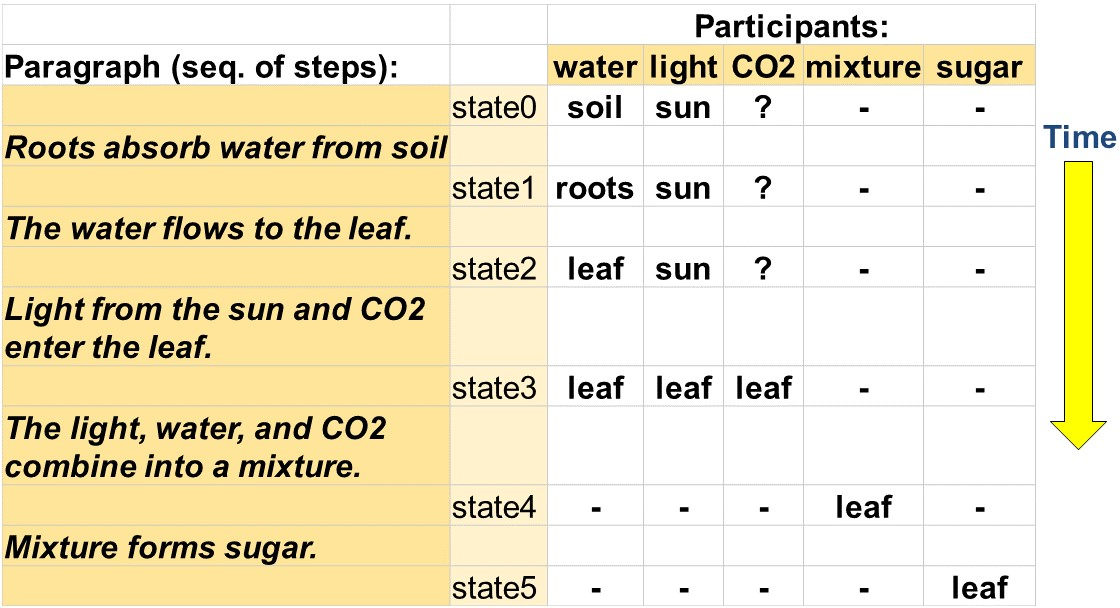
\includegraphics[width=8cm]{participant-grid-simple.JPG}
\caption{ProPara participant state change grid.}
\label{fig:participant-grid}
\end{figure}

To evaluate our system, we use the ProPara procedural text benchmark 
which contains 488 crowd-sourced paragraphs and 3100 sentences total. 
This data set is comprised of procedural text paragraphs covering different 
topics together with a human annotated table that describes the state 
(location and existence) of entities in this paragraph. Figure 
\ref{fig:participant-grid} shows an instance of the training data which 
constitutes of a paragraph about photosynthesis and the annotated state 
change grid. The state change grid contains information about where an 
entity (e.g. water or light) is at each step. Note that "?" indicates the 
location is unknown, and "-" indicates the entity doesn't exist during that step.

\section{Model and Implementation}

In this project we implement a model similar to ProGlobal, which was 
introduced in Dalvi et. al. The key feature of this model is that it predicts 
the state of \textit{all} participants at each timestep (even if the participant is 
not mentioned in a sentence). Therefore the persistence of the states are 
tracked by the model itself. 

\begin{figure}[h]
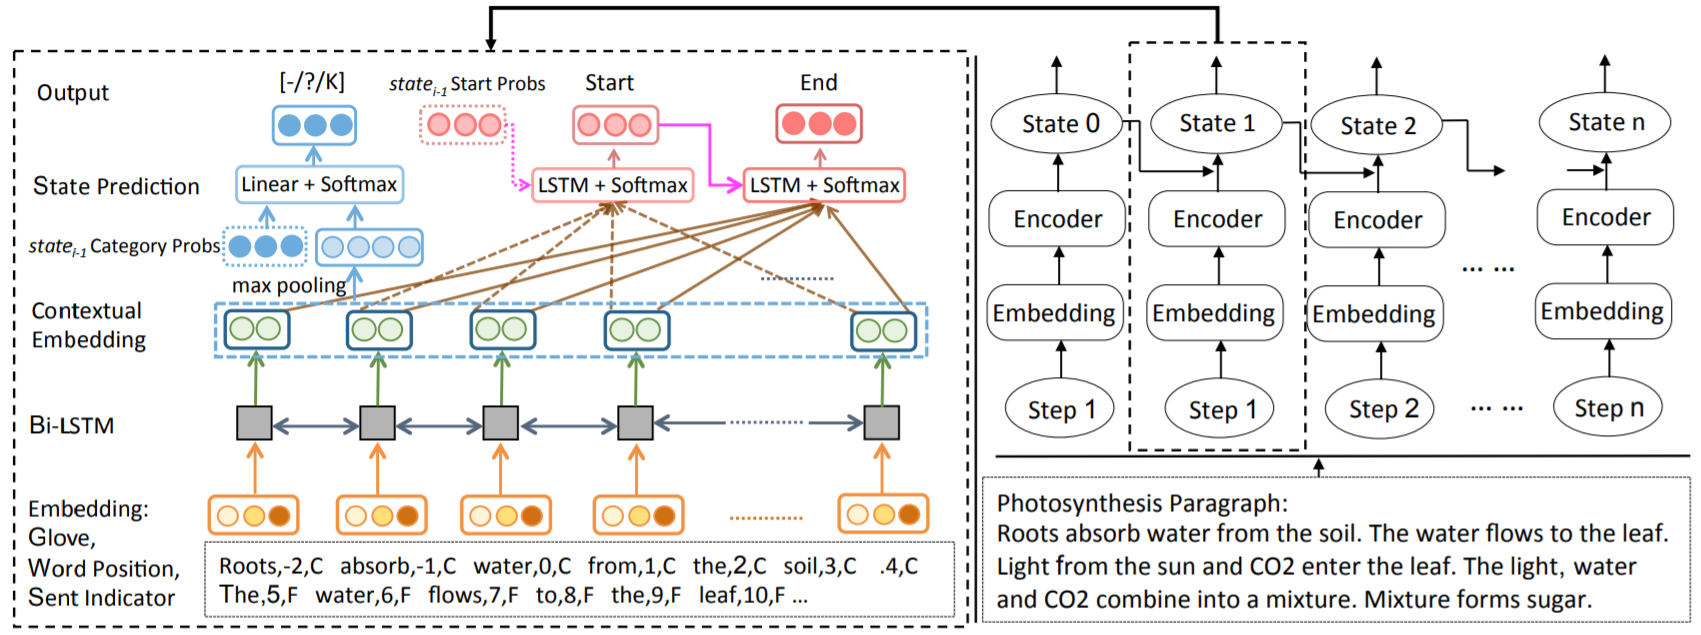
\includegraphics[width=\linewidth]{proglobal.PNG}
\caption{Diagram describing the ProGlobal model. The input of the model is the whole paragraph, plus features indicading the current sentence and the distance to the participant. Previous step predictions are fed to next step prediction}
\label{fig:participant-grid}
\end{figure}

Attention in proglobal is more complicated than that of a simple seq2seq architecture, due to the fact that proglobal is more complex. A bidirectional lstm learns a hidden global state H for each paragraph. This hidden state is then passed to various submodules.

The architecture works as follows. For each sentence in each paragraph, learn information about a participating entity, e.g. water. First, a decision is made as to the state of the entity in a sentence, e.g. exists, notexists, or unknown. If exists, then infer the location of the entity, e.g. “water is in the ground”.

The existential submodule arguably does not use attention, as it takes softmax(H) as input. On the other hand, the location submodule receives the full paragraph hidden state. We note that the visualizations show the value of every word in every timestep. However, the model only considers words within each timestep (in other words it does not look ahead to future sentences to infer location).

\section{Evaluation and Results}

During testing the system will 4 categories of questions from the output 
state change grid: 

\begin{enumerate}
  \item What are the Inputs? That is, which participants existed before the 
  	  procedure began
  \item What are the Outputs? That is, which participants existed after 
	  the procedure ended?
  \item What are the Conversions? That is, which participants were 
  	  converted to which other participants?
  \item What are the Moves? That is, which participants 
	   moved from one location to another?
\end{enumerate}

Note that these questions are templated, meaning they can be deterministically 
answered using the output state grid. The evaluation code was made available 
at \url{https://github.com/allenai/aristo-leaderboard/tree/master/propara} by 
the AI2 team. The code outputs precision, recall and F1 score for each 
question category.

\begin{table}[t!]
\begin{center}
\begin{tabular}{|l|ccc|}
\hline  \bf Model &  \bf Precision &  \bf Recal &  \bf F1 \\ \hline
ProLocal & \bf 77.4 & 22.9 & 35.3 \\
ProGlobal & 46.7 & \bf 52.4 & 49.4 \\
ProStruct & 74.2 & 42.1 & \bf 53.7 \\
\hline
\bf Our Results & 76.9 & 25.0 & 37.7 \\
\hline
\end{tabular}
\end{center}
\caption{ Results on test set. }
\end{table}


\begin{figure}[h]
  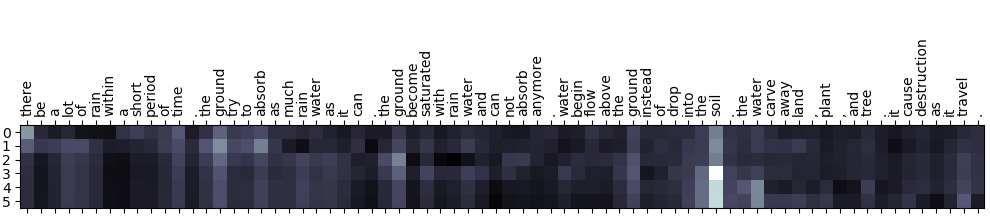
\includegraphics[width=\linewidth]{images/rain.png}
  \caption{Rain}
  \label{fig:boat1}
\end{figure}

For “rain”, the network infers the location “there” in the first sentence. This is an interesting artifact of this neural model It assumes that it has to tie a location to a word. “there” seems odd, but can be interpreted as technically correct. This is a limitation of the problem as it is set up, and not anything with the architecture itself.

The model infers that “rain” is in the ground in sentences 2 and 3. Sentence 4 is complicated, in that it is ambiguous. The water divides itself, now being both in and above the soil. The model actually infers that the water goes from the “ground” to the “soil”, not realizing that this is the same thing. From a commonsense perspective however, the correct answer seems to be “above the ground”. The negation of “instead” seems to be ignored by the model. It is clear that “soil” is overwhelmingly preferred by the attention mechanism. Perhaps because it is close in embedding space to “rain”? 

\begin{figure}[h]
  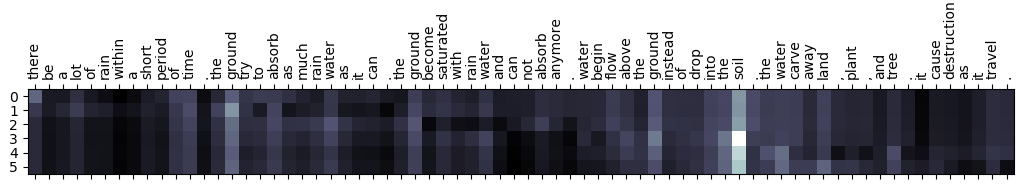
\includegraphics[width=\linewidth]{images/plant.png}
  \caption{Plant}
  \label{fig:boat1}
\end{figure}

The model infers that “plant” appears in the last sentence, and is in the soil. I have no interpretation for this, as “soil” does not appear in the last sentence. Because this network is recurrent however, the overwhelming weight on “soil” must force the model to choose this location. “tree” (not shown) looks very identical to “plant”, but the models infers that it is never introduced into a location.

\begin{figure}[h]
  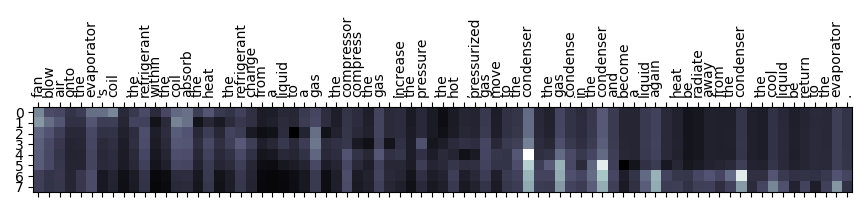
\includegraphics[width=\linewidth]{images/heat.png}
  \caption{Heat}
  \label{fig:boat1}
\end{figure}

The model infers heat’s path is “fan -> fan -> null -> condenser -> null -> condenser -> null”
This thrashing is interesting, and it doesn’t follow the narrative in the paragraph. The correct trajectory should be “air -> coil / gas / refrigerant”. Clearly there is no commonsense here, the model seems to have a high prior for “condenser” and is overwhelmingly selecting this location. There is no commonsense of temporal stability either, in that it seems unreasonable for the location to fluctuate as it does. 


\begin{figure}[h]
  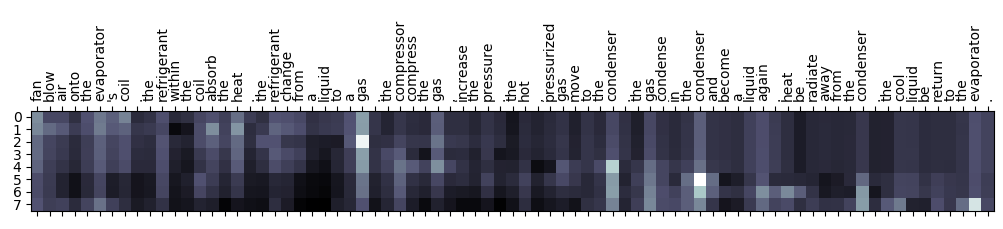
\includegraphics[width=\linewidth]{images/liquid.png}
  \caption{Liquid}
  \label{fig:boat1}
\end{figure}

To further illustrate this point, the model infers that liquid is at “gas” in sentence 3. This can almost certainly be attributed to a close embedding. There is no commonsense understanding that gas is not a container, nor that something cannot be liquid and gas.

\section{Conclusion}

It is clear that the problem of reasoning on a human level about these types of causal narratives is elusive. Can this model be said to be performing commonsense reasoning? Is this model useful in any sense? Can DL ever solve these problems? Is this a useful empirical evaluation?

The evaluation itself is oversimplified. This is almost certainly in order to make backprop more tractable while still appearing to be getting interesting results. The constraint on one span per transformation is evidence of this. This is simply unreasonable. An elaborate discussion on this matter can be found here: https://towardsdatascience.com/the-emperors-new-benchmarks-8fe8f170923b.
Suffice it to say, the system will never grasp the complexity of the intended reasoning domain. This paper seems to show that neural networks can learn arbitrarily complex functions. That’s it. The problem is that the function being learned in this situation isn’t inherently useful (it will probably not generalize to other data of this sort).

How general is the ProGlobal model architecture? It does seem to be making some effort to be globally generally. Its assumptions are that there are objects, and their locations should be tracked. It is assuming some sort of persistence and continuation. In this sense it does seem to reasonably model a low level of causal understanding. Perhaps more deductive reasoners can be placed on top of this information to produce more intuitive and interesting results. It seems reasonable to question whether this will actually work, however. There seems to be a need for commonsense reasoning even at this low level in order to prevent some of the nonsensical conclusions.

%\bibliography{emnlp2018}
%\bibliographystyle{acl_natbib_nourl}

\end{document}
